\documentclass[10pt]{article}
\usepackage[letterpaper,margin=1in]{geometry}
\usepackage{mathptmx}
\usepackage{amsmath,amssymb}
\usepackage{graphicx}
\usepackage{booktabs}
\usepackage{array}
\newcolumntype{L}[1]{>{\raggedright\arraybackslash}p{#1}}
\usepackage{xcolor}
\usepackage{tikz}
\usetikzlibrary{arrows.meta,positioning,fit,backgrounds,calc}
\usepackage{caption}
\captionsetup{font=small,labelfont=bf}
\usepackage[round,authoryear,sort&compress]{natbib}
\setlength{\bibsep}{2pt}
\usepackage[colorlinks=true,linkcolor=blue!60!black,citecolor=blue!60!black,urlcolor=blue!60!black]{hyperref}
\sloppy
\setlength{\emergencystretch}{3em}
\renewcommand{\thetable}{S\arabic{table}}
\renewcommand{\thefigure}{S\arabic{figure}}
\renewcommand{\thesection}{S\arabic{section}}

\title{\bfseries Supplementary Material for\\
``From Embodied Experience to Persistent Experience-Derived State: An Auditable Unified-Graph Architecture and a Preregistered Boundary Analysis of Activation-Based Access''}
\author{}
\date{}

\begin{document}
% The official class prints \theabstract unconditionally in \maketitle;
% supplementary material has no abstract -> define it empty.
\long\gdef\theabstract{}
% Supplementary tables are wider than the class' 5cm-left-sidebar text
% block; relax to a symmetric block (document-level geometry only; the
% class file is untouched).
\newgeometry{left=2.5cm,right=2cm,top=2.25cm,bottom=2.25cm}
\maketitle

\section{Terminology, Evidence Levels, and Protocol Layers}
\label{s1:term}

\paragraph{Terminology.} \emph{Experience}: a temporally ordered action--observation stream with timestamps and settlement outcomes. \emph{Relational knowledge}: typed assertions encoded as graph nodes and typed, weighted directed edges---distinct from raw log entries and vector embeddings. \emph{Write-back}: the pipeline step that converts experience fragments into candidate relations and promotes them into persistent structure; it is the \emph{only} pathway from experience to knowledge in FAS. \emph{Persistent}: structure survives session/episode boundaries, with runtime load (activation values) inherited along with it. \emph{Reuse}: existing structure relevant to a new situation is re-lit and enters the cognitive working set. \emph{Functional consumption}: stored knowledge enters action selection through an explicit consumer mechanism---not ``knowledge exists'' but ``knowledge changes behavior.''

\paragraph{Production and experimental paths.} To avoid confusion, all evidence is attributed to four layers, labeled at each occurrence: \textbf{P1 production default path}---zero-LLM subject behavior (graph, activation, ledger, modulation, intention loop, replay gate) runs with production configuration in the sandbox. \textbf{P2 production mechanism, assembled validation}---ledger (Exp.~C) and event framework (\texttt{enabled=False}): the mechanism lives in production code; differences are exposed by experimental assembly. \textbf{P3 mechanism-isolation layer}---the core incremental-value campaign and the relation-direction diagnosis: controlled mechanism experiments on reference models distilled from production semantics; no behavioral benefit in the production loop is claimed or required. \textbf{P4 experimental-layer harness}---the LLM decision head (not attached to production).

Two assembly audits are reported as such. (i) An early ablation matrix ran on an assembly missing the diffusion executor (the continuous-cognition loop was not wired), so its zero differences only support ``completion-level insensitivity to activation''; after repair, access-layer experiments carry the mechanism evidence. (ii) The first routing harness never built edges, swallowed 521/521 exceptions, and always produced an empty first-step focus---it was declared invalid and rebuilt and re-run (Section~S11); a later audit additionally found that the production answer pipeline originally did not render attention/demand annotations, and it has since been wired to the same cognitive structure, aligning production and harness paths on annotation rendering---this alignment fixes the reporting definition but changes no experimental number. Combined constraint: mechanism- and assembly-level evidence fully supports this paper's claims, but no ``production superiority'' statement may be extrapolated from it.

\begin{table}[h]
\centering\small
\caption{Evidence levels $\times$ protocol layers (full merged scale; Table~1 of the main text is the abbreviated version).}
\label{tab:s-evidence}
\begin{tabular}{L{3.4cm}L{4.8cm}L{6.4cm}}
\toprule
\textbf{Level} & \textbf{Meaning of a claim at this level} & \textbf{Layer the evidence comes from} \\
\midrule
L1 representational & learned structure exists and re-activates & P1 (production default path, zero-LLM) \\
L2 mechanism & measurable activation/ledger dynamics & P2 (assembled validation) and P3 (mechanism isolation on reference models) \\
L3 behavioral & stored knowledge changes action selection & P2 consumer assemblies; P4 decision-head harness (exploratory) \\
L4 general capability & --- & \emph{explicitly not claimed anywhere} \\
\bottomrule
\end{tabular}
\end{table}

\section{Internal Code-Name Mapping}
\label{s2:codes}
Historical run-family codenames appear in archived filenames and statistics files. Table~\ref{tab:s-codes} maps them to the neutral names used in the paper; the main text avoids them.

\begin{table}[h]
\centering\small
\caption{Internal code-name mapping (for navigating the archives; not used in the main text).}
\label{tab:s-codes}
\begin{tabular}{L{3.6cm}L{4.6cm}L{6.6cm}}
\toprule
\textbf{Internal code} & \textbf{Neutral name} & \textbf{Note} \\
\midrule
A10 & beacon task & information-asymmetry closed-book task (main text Section~5.1) \\
B0/B1/B2 (writeback) & write-back isolation lineages & B2 here = write-back-on lineage; \emph{do not conflate} with B2 below \\
B2 (core incremental value) & flat path-product baseline & closed-form flat baseline of the mechanism campaign; distinct meaning from the writeback lineage \\
B2 (diffusion\_b2) & four-condition access family & a third use of the label, historical \\
B1 (core incremental value) & direct injection baseline & graph-free control \\
B3 / B4 & random activation / oracle & equal-energy control; generator-correctness precheck \\
C-1..C-4 & preregistered conditions 1--4 & the four confirmatory topologies of the mechanism campaign \\
O1--O3 & topology detectors O1--O3 & O3 = shared-hub (combinational) topology \\
D-flat / D-noact & embedding-retrieval / activation-off controls & beacon and routing conditions \\
D (event framework) & event-framework experiment & assembled validation of the production-default-off channel \\
C20e / C20g & event-framework follow-ups & real-failure-receipt variants \\
C-emo & affective dose experiment & scalar modulation dose response \\
D-CI & intention lifecycle experiment & continuous-intention formation through decay \\
F (hebbian) & Hebbian isolation & weight-level isolation, behavior sub-threshold \\
G0/G1/G2 & re-activation conditions & full graph / episodic-stripped / clean \\
H/K/L (longchain) & long-chain variants & L0 full, L1 $-$diffusion, L2 $-$write-back, L3 $-$priors, L3b prior restored \\
I/U (envchange) & environment-change family & scale insufficient; re-validation probes \\
J/P (prior\_boundary) & prior-level family & P0 zero priors, P1 mechanics tables only, P2 full \\
M1--M3 (minecraft) & live sessions & observational only \\
T1--T4 (campaign) & mechanism topologies & 3in/100n/25\% to 5in/1000n/75\% \\
T1--T4 (routing) & decision-head task classes & knowledge reuse / interference / re-routing / competing targets \\
I1--I3 (relation dir.) & injection conditions & single, single, dual input \\
F / B (relation dir.) & forward / bidirectional projection & production graph vs.\ +reverse-edge projection \\
A/B closure & closure-masking checks & completion-layer insensitivity instances \\
\bottomrule
\end{tabular}
\end{table}

\section{Experiment Families and Archival Census}
\label{s3:families}

Every run is archived by the run recorder (metadata, event stream, start/end graph snapshots, metrics) into content-addressed directories. The archival census of behavioral families totals 494 runs (ablation 77, eventframe 53, sandbox 43, ci 34, transfer 32, reuse\_a2 31, prior\_boundary 31, longchain 29, reuse 28, emotion 25, hebbian 24, event\_transfer 22, diffusion\_b2 22, envchange 14, diffusion 12, baselines 8, prior\_conditions 7, minecraft 2); further, the mechanism campaign comprises 34,016 runs (line-countable in its raw results file), the beacon campaign 80, the routing campaign 520, the relation-direction diagnosis 60, and the falsification campaign 663; the shared-hub parameter sweep (Section~S8) adds 2,550 runs. Failures and pilots are all retained.

\begin{table}[h]
\centering\small
\caption{Family $\rightarrow$ paper-section provenance.}
\label{tab:s-family}
\begin{tabular}{L{4.6cm}L{3.6cm}L{6.6cm}}
\toprule
\textbf{Family (internal code)} & \textbf{Main-text section} & \textbf{Purpose / headline number} \\
\midrule
Beacon (A10) & \S5.1 & information asymmetry: 20/20 vs 0/20 vs 0/20 vs 20/20 \\
A2 / reuse & \S5.2 & 8-round promotion of 4 relations per seed \\
B0/B1/B2 (writeback) & \S5.2 & write-back isolation 0 vs 13 nodes \\
G0/G1/G2 & \S5.2 & cross-context re-activation 4/12--0/8--0/0 \\
Exp.\ C (transfer) & \S5.2 & ledger channel 13 vs 16 ticks \\
Exp.\ D / C20e/C20g & \S5.2 & event-framework channel @6 vs @9, @15 vs @17 \\
Exp.\ B (diffusion) & S7 & access-layer separation (post-assembly-fix) \\
B2 (diffusion\_b2) & S7 & four-condition separation 61.5/16.6/45.8/17.2 \\
falsification & \S5.3 & 663 runs: JCG$>0$ rate 0.970, hypothesis-group MRR@1$=1.0$ \\
core incremental value & \S5.3, S7 & 34,016 runs: C-1..C-4, combo, sweeps, counterfactuals, oracle \\
shared-hub sweep (new) & \S5.3, S8 & 2,550 runs: 84-cell grid + O3 replication \\
C-emo (emotion) & \S5.4 & dose response 49.8/52.5/57.4 \\
D-CI (ci) & \S5.4 & intention lifecycle 3--4 per run; expression unattained \\
F (hebbian) & \S5.4 & Hebbian weight isolation $+0.074$; behavior sub-threshold \\
H/K/L (longchain) & \S5.4 & 315 / 259 / 0-of-5 / 315 ticks \\
J/P (prior\_boundary) & \S5.4 & P0 0/25; P1$=$P2 25/25 \\
I/U (envchange) & S12 & environment-change scale insufficient \\
M1--M3 (live) & \S5.4 & observational forms; live causal ledger \\
A/B matrix (ablation) & S1 & completion-layer masking \\
routing v1 (invalid) & S11 & declared invalid; not a basis for claims \\
routing v2 & \S5.4, S11 & 520 runs, exploratory boundary \\
relation direction & \S5.3, S9 & direction-semantics mechanism diagnosis \\
determinism re-run (new) & \S5.5, S10 & 20 re-runs: outcomes 20/20, trajectories 7/20 \\
\bottomrule
\end{tabular}
\end{table}

\emph{Provenance notes.} (i) The mechanism campaign's primary numbers use the independent 663-run falsification campaign's statistics as the reference-model source; a directory named \texttt{experiments/mechanism\_campaign} is a \emph{different}, later activation-landscape audit whose probes failed and whose formal runs never executed---it is not a number source. (ii) The routing campaign's first statistics file was renamed with an INVALID suffix and documented; the current statistics file is the official v2 campaign.

\section{Component Status}
\label{s4:components}

\begin{table}[h]
\centering\small
\caption{Component status (implementation / experimental validation / evidence level / default switch).}
\label{tab:s-components}
\begin{tabular}{L{3.6cm}L{1.9cm}L{2.6cm}L{1.2cm}L{4.6cm}}
\toprule
\textbf{Component} & \textbf{Impl.} & \textbf{Validated} & \textbf{Level} & \textbf{Notes / default} \\
\midrule
Unified graph (single graph, 7 label classes, 8 relation types, negative weights) & production & all experiments & L1 & auxiliary layers never build structure \\
Spreading activation (decay/gain/suppression/Top-$k$/emit-as-transfer) & production & access tasks, four conditions & L2 & runs every tick \\
Evidence-weighted write-back (window/\allowbreak support/\allowbreak confidence/\allowbreak promotion) & production & isolation, reuse, event exps & L1/L2 & sole structure-writing channel \\
Persistence and inheritance (structure + activation) & production & re-activation, ledger exps & L1/L2 & cross-episode; snapshot rotation + shrink guard \\
Ledger consumers (reward ledger + trial ledger) & production & transfer exp & L3 & prior bonus $\pm0.05$ \\
Event framework (polarity-slot edges) & implemented & event exps (assembly) & L2/L3 & \textbf{production default OFF} \\
Affect/neuromodulation (graph citizens: tonic truth, derived level, graph as effect source) & production & dose exp & L2 & every tick \\
Hebbian co-activation & production & isolation exp & L2 & default on; behavior sub-threshold \\
Intention lifecycle & production & lifecycle exp & L2 & expression level unvalidated \\
Offline experience replay gating & production & not touched in this paper & --- & idle gating \\
Episodic buffer (capacity/\allowbreak forgetting/\allowbreak retrieval/\allowbreak promotion) & production & not touched in this paper & --- & short-horizon integration layer; promotes tags only \\
Web-search action node & production & not touched in this paper & --- & external knowledge acquisition \\
Hormone graph citizenship (tonic real value, derived level, graph as effect source) & production & not touched in this paper & --- & hormone \emph{direct behavioral} control not implemented \\
LLM decision head & experimental & routing campaign, 520 runs & L3 (exploratory) & not attached to production \\
Prospective memory, full perception pipeline, symbolic reasoning, RL policy nodes & not implemented & --- & --- & future work \\
\bottomrule
\end{tabular}
\end{table}

\section{Write-Back: Worked Example, Taxonomy, and Claim Audit}
\label{s5:wb}

The full promotion list of the write-back-on lineage (15 relations) and the corresponding graph snapshots ship with the artifacts. Example promotion (seed 1): \texttt{gather\_resource(oak\_log)} leads-to \texttt{change:inventory:oak\_log:count\_increased}, cumulative support 8 / confidence 0.889 after 8 rounds, both endpoints mark-activated on write.

\begin{table}[h]
\centering\small
\caption{Write-back-lineage (seed 1) 15 promoted-relation taxonomy. Classification by edge content; the two window-polluted pairs are a subset of the substantive class.}
\label{tab:s-taxonomy}
\begin{tabular}{L{6.6cm}L{2.2cm}L{5.2cm}}
\toprule
\textbf{Promoted relation} & \textbf{Class} & \textbf{Reading} \\
\midrule
\texttt{gather\_resource(oak\_log)} $\rightarrow$ \texttt{change:inventory:\newline oak\_log:count\_increased} & substantive & mining yields items \\
\texttt{gather\_resource(oak\_log)} $\rightarrow$ \texttt{change:block:\newline oak\_log:disappeared} & substantive & mining removes blocks \\
\texttt{craft\_item(oak\_planks)} $\rightarrow$ \texttt{change:inventory:\newline oak\_log:count\_decreased} & substantive & crafting consumes logs \\
\texttt{craft\_item(oak\_planks)} $\rightarrow$ \texttt{change:inventory:\newline stick:count\_decreased} & substantive & crafting consumes sticks \\
... (7 further inventory/block pairs) & substantive & \\
\midrule
\texttt{gather\_resource(oak\_log)} $\rightarrow$ \texttt{change:inventory:\newline oak\_planks:count\_increased} & substantive, window-polluted & downstream craft attributed to upstream gather \\
\texttt{gather\_resource(oak\_log)} $\rightarrow$ \texttt{change:inventory:\newline stick:count\_increased} & substantive, window-polluted & same \\
\midrule
\texttt{$\{A\}$} $\rightarrow$ \texttt{change:self:\{A\}:succeeded} ($\times 4$) & degenerate & action $\rightarrow$ own success; tautology \\
\bottomrule
\end{tabular}
\end{table}

\begin{table}[h]
\centering\small
\caption{Implementation $\rightarrow$ claim audit (excerpt; the full 17-claim audit ships with the artifacts). Verdicts: S = mechanism exists and is experimentally verified; Q = qualified/assembly-level; U = unsupported and reported as such.}
\label{tab:s-audit}
\begin{tabular}{L{4.6cm}L{3.2cm}L{3.6cm}L{1.7cm}}
\toprule
\textbf{Claim} & \textbf{Key implementation} & \textbf{Audit notes} & \textbf{Verdict} \\
\midrule
S1 experience $\rightarrow$ new relational structure under scaffolding & attribution pipeline (scoring / aggregation / promotion) + write-back switch & 4 degenerate + 2 window-contaminated are self-reported artifacts; code matches & S \\
S2 persistence and cross-context re-activation & graph save/load + snapshot rotation + shrink guard & 4/12 carried by episodic structure (access layer) & S \\
S3 ledger channel changes action selection & reward/trial ledgers $\rightarrow$ candidate prior bonus & difference lands at action-selection layer, not completion layer---matches paper's self-scope & S \\
S4 event framework changes action selection & settlement write-back; \texttt{enabled=False} (config) & audit confirms production-default off, zero graph writes & S (assembly) \\
S5 scalar modulation of propagation dynamics & internal-state tonic/level; modulator as graph citizen; projection & graph is the effect source; dose-response gate ran & S \\
S6 mechanics tables necessary; zero-prior lock & mechanics tables + goal system & P0 locks at unreachable goal = upstream experience-generation failure; behavior matches code & S \\
S7 relation direction limits propagation & directed graph; 8 bidirectional whitelist vs forward; recipe edges sinkified & independent re-check $\rho$ .33$\rightarrow$.65, $r{=}.886$, 10/10; no behavioral test; production graph unmodified & S (mechanism) \\
Q1 diffusion produces a distinct access pattern (not behavior) & diffusion engine (step/emit) & independent falsification campaign: 663 runs, JCG$>0$ 0.970 & Q \\
U2 semantic write-backs consumed by planner & planner does not read semantic write-back graph & code audit: no consumption path & U \\
U5 routing robustly better than baselines & routing harness & 520/520 valid; competing-targets raw $p{=}.046$, corrected $p{\approx}1$; tokens 2.1--3.7$\times$ & U (directional) \\
(extra) production answer pipeline renders attention/demand & annotation rendering switch (wired after audit) & audit-identified definitional gap repaired; rendered as projection references, values not exposed & fixed \\
\bottomrule
\end{tabular}
\end{table}

\section{Beacon Task: Case Study and Embedding-Baseline Check}
\label{s6:beacon}

\begin{figure}[h]
\centering
\resizebox{\textwidth}{!}{%
\begin{tikzpicture}[
  bn/.style={draw, rounded corners, align=center, inner sep=6pt, font=\scriptsize},
  sc/.style={bn, fill=blue!8}, wb/.style={bn, fill=orange!12}, ob/.style={bn, fill=gray!8},
  res/.style={bn, fill=green!10}, neg/.style={bn, fill=red!6},
  flow/.style={-{Latex}, semithick}, note/.style={font=\scriptsize, gray!50, align=center}]
\node[sc] (prac) at (0,0) {practice phase (8 rounds)\\ \scriptsize \strut action--observation stream\strut};
\node[wb] (wbk) at (0,-2.1) {write-back (attribution pipeline)\\ \scriptsize \strut \texttt{gather\_resource(oak\_log)} leads-to ($w{=}0.889$)\\ \scriptsize \strut \texttt{change:inventory:oak\_log:count\_increased}\\ \scriptsize \strut support 8, confidence 0.889, promotion + mark-active\strut};
\node[sc] (gra) at (0,-4.6) {persistent unified graph (structure + activation inheritance)};
\draw[flow] (prac) -- (wbk); \draw[flow] (wbk) -- (gra);
\node[ob] (bk) at (9.5,0) {beacon task (closed-book, n=20)\\ \scriptsize \strut recipe only in memory, menu gating, facts stripped\strut};
\node[res] (fas) at (5.6,-2.3) {\textbf{fas\_full}:\\ persistent graph + activation context\\ 20/20 completed ($\bar{x}$ decisions 2.15)\\ first action \texttt{gather\_oak\_log} 20/20};
\node[res] (dflat) at (14.0,-2.3) {\textbf{D-flat}:\\ embedding-retrieval control\\ 20/20 completed ($\bar{x}$ decisions 2.1)};
\node[neg] (dno) at (7.2,-4.6) {\textbf{D-noact} 0/20\\ structure present, runtime absent};
\node[neg] (dir) at (12.2,-4.6) {\textbf{llm\_direct} 0/20\\ no memory context};
\draw[flow] (bk) -- (fas); \draw[flow] (bk) -- (dflat);
\draw[flow] (bk) -- (dno); \draw[flow] (bk) -- (dir);
\draw[flow] (gra.east) to[out=0,in=190] (bk.west);
\node[note] at (9.3,-5.9) {McNemar exact: fas vs direct $p{=}2\times10^{-6}$; fas vs D-noact $p{=}2\times10^{-6}$;\\ fas vs D-flat $p{=}1.0$ (decision Wilcoxon $p{=}0.72$)---\emph{persistent relational reuse supported;}\\\emph{activation necessity not supported}.};
\end{tikzpicture}}%
\caption{A complete real case study: the wood-to-plank chain from practice experience, through evidence-weighted write-back into persistent graph structure, to the behavioral benefit in the information-asymmetric beacon task. All numbers from the archived beacon analysis (80 runs, four conditions $\times$ 20 paired seeds).}
\label{fig:s-case}
\end{figure}

\paragraph{What kind of retriever is D-flat?} D-flat is a genuine sentence-embedding retriever: it encodes all graph node identifiers with a public, locally runnable sentence-transformer model (BAAI/bge-small-zh-v1.5) and ranks them by cosine similarity to the task text---no activation, no propagation, no path structure. We verified this at import level (the retrieval path instantiates the embedding provider and computes normalized cosine similarities; no diffusion call is reachable from it).

\paragraph{Zero-LLM accessibility check.} Design (frozen before execution): rebuild the beacon step-0 assembly for each of the 20 paired seeds (production graph-building path with the recipe closure; no observations ingested), compute the full-graph embedding similarity ranking for the exact goal text used in the campaign, and record the ranks of the recipe and resource nodes. Result: the graph is identical across all 20 seed assemblies (44 nodes; deterministic construction); \texttt{item:oak\_planks} ranks \textbf{2nd} and \texttt{item:oak\_log} ranks \textbf{4th} in every assembly---both inside the Top-8 context window that D-flat presents to the decision head. This is the enabling condition of D-flat's 20/20 result, verified without any LLM call. (Purely descriptive; no statistical test applies to a single deterministic assembly state.)

\section{Activation Mechanism: Access-Layer Separation}
\label{s7:activation}

\emph{Four-condition access task ($n{=}5$, deterministic).} On an access task---diffusion on; diffusion off ($\beta{=}0$, injection only); random-activation control (same energy injected into random semantic nodes); retrieval-oracle control (target-chain nodes raised every tick)---full diffusion produces activation quality 61.5 over a field of 39 lit nodes; diffusion off 16.6 over 17; the random control is comparable in quality (45.8) but with a larger, structureless field whose out-of-sight targets light at drift moments (ticks 1--9 across seeds) rather than in a fixed pattern; the oracle 17.2 over 18 (Fig.~\ref{fig:s-diffusion}). Structural diffusion is therefore distinguishable from both noise and lookup at the knowledge-access layer.

\emph{Companion causal experiment (re-run after the assembly repair).} Gap ``pointed-at'' entity activation 1.5$\rightarrow$5.0 capped (control wanders 1.1--1.7); \emph{out-of-sight} pure-diffusion signal \texttt{oak\_log} 0.43 vs 0.0; gap-source energy drains under emit-as-transfer (1.43$\rightarrow$0.16) while the control sticks; 2-hop lit field 5 vs 4. Completion layer: zero difference in both experiments (closure masking; main text Section~5.4).

\emph{Mechanism-campaign ancillary results.} B1 direct injection and B3 random activation confirm the contrast setup works independently of the graph; the B4 oracle precheck (MRR$=1.0$ on all four topologies) excludes generator-side error. Hidden oracle (30 seeds, label/ID permutation): target rank 22.5 unchanged. Insertion order: 10 permutations, CV$=0.0$. Counterfactual C2 (no joint target): all four methods 0.0. Negative-edge test: joint top-1 0.0333$=$0.0333, total score 17.41 unchanged (no collapse).

\begin{figure}[h]
\centering
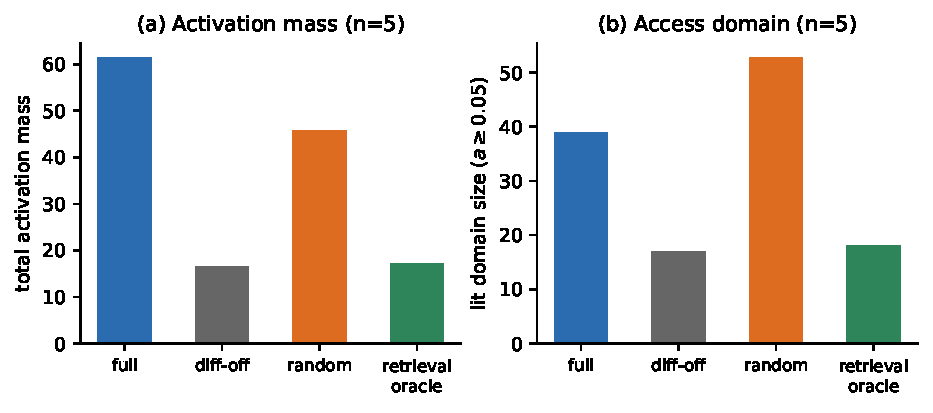
\includegraphics[width=\textwidth]{figures/fig_diffusion.pdf}
\caption{Four-condition activation task ($n{=}5$, deterministic). Structural diffusion produces a distinct access field; same-energy random activation cannot reproduce it; the target-chain oracle is narrower.}
\label{fig:s-diffusion}
\end{figure}

\emph{Per-condition confirmatory numbers (preregistered, $n{=}50$ paired seeds each).} Median $\Delta$JCG: $-0.402$ (C-1), $-0.402$ (C-2), $-0.784$ (C-3), $-0.782$ (C-4); reverse-direction one-sided Wilcoxon with Holm correction $p{=}1.5\times10^{-9}$ (the frozen implementation's one-sided $p$ is half the two-sided $p$ regardless of direction; the preregistered-direction tail is its complement, ${\approx}1$; see main \S4.2); effect $r{=}0.615$; seeds where FAS beats flat: 0/200. MRR (FAS vs flat path-product): 0.0435/0.0426 vs 0.5/0.5 on the two smaller topologies; tie at 1.0 on the two larger. Robustness sweep: slope 0.0076 (flat 0.0), AUC 0.0427 vs 0.04, critical noise 0.0$=$0.0. Weight sweep: both methods reach MRR$=1.0$ together at $w{=}0.7$ (FAS 0.083@0.5 $\rightarrow$ 1.0@0.7; flat 0.077 $\rightarrow$ 1.0).

\section{Shared-Hub Parameter Sweep: Design and Full Data}
\label{s8:sweep}

\paragraph{Design (frozen before execution).} Question: where in (edge weight $w$, converging-input count $k$, private-path depth $d$) does activation-based access beat the closed-form flat baseline on the shared-hub structure? Topology per cell and seed: $k$ inputs, each connected by $d$ private hops (edge weight $w$) to a shared hub, one hop ($w$) to the joint target T; each input also has a 2-hop private path (weights 0.8/0.8, fixed, mirroring the original shared-hub design's branch strength) to a single target $S_i$; each input carries 4 two-hop distractors (weight 0.3), 2 of them in the candidate ranking domain; candidates $=$ $\{T\} \cup \{S_i\} \cup$ distractors. Grid: $w\in\{0.3,\ldots,0.9\}$ (7) $\times$ $k\in\{2,3,4,6\}$ (4) $\times$ $d\in\{0,1,2\}$ (3) $=$ 84 cells, 30 paired seeds per cell; plus an exact replication cell of the original shared-hub configuration ($k{=}2$, $d{=}0$, $w{=}0.5$, no distractors) as a hard preflight. Diffusion parameters identical to the preregistered campaign (steps $=$ joint hops $+ 2$; seed strength 5.0; ratio 0.5; emit-as-transfer 1.0; decay 0.05; cap 5.0). Metrics: success@1 on T (primary), MRR, JCG. Statistics: per-cell paired exact McNemar (success) and two-sided Wilcoxon (MRR); the sweep is \emph{descriptive}---no universal multiple-comparison correction is applied, and no single-cell $p$ is used confirmatorily; the paper cites only sign-consistent cell counts and the surface shape. Failing-test criterion (declared in advance): if no cell shows FAS strictly better, the paper's wording reverts to ``the single-cell positive difference found no parameter-region support.'' A design correction (v1.1, before any formal run): $d$ was initially mis-specified, which made the original configuration unreachable in the grid; the preflight failed as designed, $d$ was redefined as private-hop count with range $\{0,1,2\}$, and the corrected design was frozen before any data was produced.

\paragraph{Results (2,550 runs).} Preflight replication: FAS 30/30 vs flat 0/30 (McNemar $p{=}1.9\times10^{-9}$)---the original single-design finding reproduces exactly. Grid: FAS strictly better in \textbf{11/84} cells, flat strictly better in \textbf{9/84}, tie in 64.

\begin{table}[h]
\centering\small
\caption{Cells where FAS is strictly better (success@1 over 30 seeds; all at $w{\le}0.5$ and $d{\le}1$).}
\label{tab:s-sweepwin}
\begin{tabular}{lllll}
\toprule
$k$ & $d$ & $w$ & FAS & flat \\
\midrule
2 & 0 & 0.4 & 8/30 & 0/30 \\
2 & 0 & 0.5 & 30/30 & 0/30 \\
3 & 0 & 0.3 & 30/30 & 0/30 \\
3 & 0 & 0.4 & 30/30 & 0/30 \\
4 & 0 & 0.3 & 30/30 & 0/30 \\
4 & 0 & 0.4 & 30/30 & 9/30 \\
6 & 0 & 0.3 & 30/30 & 0/30 \\
4 & 1 & 0.4 & 9/30 & 0/30 \\
4 & 1 & 0.5 & 30/30 & 0/30 \\
6 & 1 & 0.3 & 30/30 & 0/30 \\
6 & 1 & 0.4 & 30/30 & 0/30 \\
\bottomrule
\end{tabular}
\end{table}

\begin{table}[h]
\centering\small
\caption{Cells where flat is strictly better (all at $w{\ge}0.7$ and $d{\ge}1$).}
\label{tab:s-sweeplose}
\begin{tabular}{lllll}
\toprule
$k$ & $d$ & $w$ & FAS & flat \\
\midrule
2 & 1 & 0.7 & 0/30 & 30/30 \\
2 & 1 & 0.8 & 8/30 & 30/30 \\
2 & 2 & 0.8 & 0/30 & 30/30 \\
2 & 2 & 0.9 & 0/30 & 30/30 \\
3 & 2 & 0.7 & 0/30 & 30/30 \\
3 & 2 & 0.8 & 0/30 & 30/30 \\
3 & 2 & 0.9 & 0/30 & 30/30 \\
4 & 2 & 0.7 & 0/30 & 30/30 \\
4 & 2 & 0.8 & 9/30 & 30/30 \\
\bottomrule
\end{tabular}
\end{table}

On the original-configuration axis ($k{=}2$, $d{=}0$): FAS/flat success 0/0 at $w{=}0.3$, 8/0 at 0.4, 30/0 at 0.5, then 30/30 at $w\ge0.6$---flat catches up exactly when the hub-path weight reaches 0.6 (median MRR: FAS 0.33/0.50/1.00 vs flat 0.33/0.33/0.33/1.00 across $w{=}0.3$--0.6). All 84 cell-level rows, raw per-seed metrics, and the extraction script ship with the artifacts; the numbers in this section and the main text are read programmatically from \texttt{sweep\_summary.csv} / \texttt{paper\_numbers.json}.

\section{Relation-Direction Diagnosis: Full Data}
\label{s9:reldir}

\emph{Static audit} (production recipe graph, 44 nodes/53 edges): the five relation classes (produces 8 / belongs 18 / drops 13 / needs 11 / needs-tool 3) have all-sink targets (sink fraction $=1.0$); \texttt{item:*} 13/13 with zero out-edges; a depth-1 star forest; forward 2-hop reachability 0. Construct graph B $=$ production graph F $+$ 41 generic reverse projections (53$\rightarrow$94 edges, no node special-casing; sandbox-memory only, production graph zero modification). 60 runs $=$ 2 graphs $\times$ 3 injection conditions (I1/I2 single input, I3 dual input) $\times$ 10 paired seeds. All 21 paired tests give $p{=}0.001953$---the minimum attainable two-sided $p$ at $n{=}10$ (exact Wilcoxon, all seeds concordant), $r{=}0.886$, 10/10 seeds in the same direction; this certifies uniform direction, not effect size.

\emph{Main-axis numbers}: forward 2-hop reachability F always 0, B 10/9/12; 3-hop B 6; lit nodes F 6/6/9 vs B 22/21/27; rank correlation between topological score and diffusion activation $\rho$ F 0.265/0.275/0.325 vs B 0.542/0.513/0.645 (dual input: $p{=}0.002$); shared-node (\texttt{item:stick}) absolute activation (dual input) F 0.833 vs B 0.475 (single-input 0.417 vs 0.253/0.239); additive prediction 0.491 $\approx$ measured 0.475; Gini 0.417 $\rightarrow$ 0.792--0.824.

\emph{Not run, recorded as such}: the suppression-off control is unavailable because the architecture has no global negative-weight switch; no behavioral experiment this round; the production graph was not modified.

\begin{figure}[h]
\centering
\begin{tikzpicture}[
  bar/.style={draw, fill=blue!25, minimum height=0pt, anchor=south west},
  bbar/.style={draw, fill=orange!45, minimum height=0pt, anchor=south west},
  lbl/.style={font=\scriptsize},
  axis/.style={gray!60, thin}]
\node[lbl, anchor=west] at (0,2.7) {(a) 2-hop reachability (reach2 / reach3)};
\draw[axis] (0,0) -- (5.0,0);
\fill[blue!25] (0.05,0) rectangle (0.6,0.9); \node[lbl, anchor=west] at (0.4,-0.32) {F: 0};
\fill[orange!45] (1.2,0) rectangle (1.2+12*0.07,2.0); \node[lbl, anchor=west] at (1.2,-0.32) {B: 9--12 (reach2)};
\fill[orange!60] (3.4,0) rectangle (3.4+6*0.07,1.2); \node[lbl, anchor=west] at (3.4,-0.32) {B: 6 (reach3)};
\node[lbl, anchor=west] at (0,-2.15) {(b) topological alignment $\rho(\mathrm{score},\mathrm{act})$ (I3)};
\draw[axis] (0,-1.75) -- (11.0,-1.75);
\fill[blue!25] (0.05,-1.75) rectangle (0.05+0.325*8,-1.75+0.9); \node[lbl, anchor=west] at (0.05,-2.62) {F: 0.325};
\fill[orange!45] (4.2,-1.75) rectangle (4.2+0.645*8,-1.75+0.9); \node[lbl, anchor=west] at (4.2,-2.62) {B: 0.645};
\node[lbl, anchor=west] at (0,-4.45) {(c) shared-node absolute activation (\texttt{item:stick}, I3)};
\draw[axis] (0,-4.05) -- (9.0,-4.05);
\fill[blue!25] (0.05,-4.05) rectangle (0.05+0.833*6,-4.05+0.9); \node[lbl, anchor=west] at (0.05,-4.92) {F: 0.833};
\fill[orange!45] (4.2,-4.05) rectangle (4.2+0.475*6,-4.05+0.9); \node[lbl, anchor=west] at (4.2,-4.92) {B: 0.475};
\node[lbl, align=left, anchor=west] at (0,-5.7) {$\rho$ doubles but single-node activation dilutes: the bidirectional projection improves alignment\\ and coverage, not guaranteed higher shared-node absolute activation.};
\end{tikzpicture}
\caption{Relation-direction experiment summary ($n{=}10$ paired seeds; all 21 tests $p{=}0.001953$, $r{=}0.886$, 10/10 seeds same direction). (a) bidirectional projection restores multi-hop reachability; (b) topological alignment doubles under dual input; (c) shared-node absolute activation is instead lower---the benefit comes with a dilution cost.}
\label{fig:s-reldir}
\end{figure}

\section{Determinism Re-Run of the Decision-Head Family}
\label{s10:rerun}

Design (frozen before execution): re-run a 5-seed $\times$ 4-condition subset of the beacon campaign (seeds 0--4; conditions fas\_full / D-noact / D-flat / llm-direct; identical code path, fresh output directory) and compare against the archived campaign runs on success, decision counts, steps-to-craft, first action, and the full action sequence.

\begin{table}[h]
\centering\small
\caption{Determinism re-run: agreement with the archived campaign (5 seeds $\times$ 4 conditions).}
\label{tab:s-rerun}
\begin{tabular}{L{3.2cm}L{3.6cm}L{3.6cm}L{3.6cm}}
\toprule
\textbf{Condition} & \textbf{Success matches} & \textbf{First-action matches} & \textbf{Full-sequence matches} \\
\midrule
fas\_full & 5/5 & 5/5 & 3/5 \\
D-flat (embedding) & 5/5 & 4/5 & 4/5 \\
D-noact & 5/5 & 5/5 & 0/5 \\
llm-direct & 5/5 & 5/5 & 0/5 \\
\midrule
Total & 20/20 & 19/20 & 7/20 \\
\bottomrule
\end{tabular}
\end{table}

Reading: task outcomes reproduce exactly, but trajectories do not---the remote LLM endpoint is not bit-deterministic even at temperature 0 (provider-side state is outside our control). The paper therefore claims trajectory-level determinism only for the zero-LLM families; the decision-head families are outcome-robust but not trajectory-reproducible, and no claim rests on their exact trajectories.

\section{Routing Campaign: Full Results}
\label{s11:routing}

\paragraph{v1 invalidation record.} The first campaign was rejected by assembly audit before formal writing: (R1) the experimental graph had zero edges (the runner never built edges; activation only traveled existing edges); (R2) 521/521 demand/gap/routing calls threw and were swallowed into placeholder text (the ``$-$demand'' ablation was an identity); (R3) 80/80 first-step focus empty. No v1 number (including anything in earlier paper drafts) is a basis for any claim in this paper; the stale statistics file was renamed with an INVALID suffix and documented, and the current statistics file is the official v2 campaign.

\paragraph{v2 results.} The rebuilt official campaign runs on the production edge-building path: seeding a real graph (37 nodes), real observation-driven edge construction, core exceptions propagate, and 9 harness invariants are fail-fast; $5\times4\times20+3\times2\times20=520$ runs in total, all valid. Token statistics (per-decision prompt means): FAS context 1456/1084/2070/2662 (T1--T4) vs no-context 661/528/554/1267, i.e., 2.1--3.7$\times$; all 20 principal token comparisons $p\le0.003$. Mechanism telemetry (ablation family $n{=}40$): diffusion ON raises activation divergence 2.4$\rightarrow$9.9, pick precision 0.717 vs 0.734, demand annotations present 100\% vs 0\%.

\begin{table}[h]
\centering\small
\caption{Routing v2: task-level results ($n{=}20$ paired seeds, Wilcoxon; uncorrected $p$).}
\label{tab:s-routing}
\begin{tabular}{L{3.4cm}L{3.0cm}L{3.4cm}L{4.0cm}}
\toprule
\textbf{Task} & \textbf{Key contrast} & \textbf{Numbers} & \textbf{Significance (uncorrected)} \\
\midrule
T1 knowledge reuse & FAS vs direct decisions & 3.25 vs 4.2 & $p{=}0.064$ (directional fewer) \\
T1 knowledge reuse & FAS vs history & 3.25 vs 2.5 & $p{=}0.035$ (worse) \\
T2 interference suppression & all conditions completion & 20/20 & none (ceiling) \\
T3 environmental re-routing & FAS vs history / rag & 4.15 vs 2.3 / 2.8 & $p{=}0.003$ / $0.044$: slower \\
T4 competing targets & FAS vs direct completion & 19/20 vs 15/20 & $p{=}0.046$ (directional) \\
T4 competing targets & decisions & 5.45 vs 7.25 & $p{=}0.029$ \\
T4 competing targets & target utilization & 0.48 vs 0.30 & $p{=}0.010$ \\
\bottomrule
\end{tabular}
\end{table}

\paragraph{Reading.} After Bonferroni correction over the campaign's 280 tests, all three competing-targets metrics give $p{\approx}1$; that task is directional only. The positive reading is ``FAS context $\neq$ no context'' in an information-competition scenario; mechanism telemetry joined with the shared-hub analysis implicates associative recall on observation-co-occurrence subgraphs, not propagation of recipe knowledge, as the carrier. The re-routing efficiency deficit and token costs are the robust cost side. The campaign's boundary assumption (fully observable tasks $\Rightarrow$ limited marginal value of memory context) is stated in the main text, together with its untested complement (information asymmetry)---the beacon task provides the first closing evidence for exactly that complement.

\section{System-Level Details}
\label{s12:system}

\paragraph{Long chain.} A 14-step chain (13 in-recipe steps plus the documented smelting-instant-settlement simplification, a two-tool intermediary branch, decoy resources) completes 5/5 seeds at 315 ticks under full configuration (L0). Removing graph prior edges \emph{and} the smelting task prior (L3): 0/5 (65 actions / 58 redundant / 33 failed)---the agent cannot plan out-of-recipe transitions. Re-adding only the smelting prior (L3b) restores the bit-identical 315 ticks. $-$diffusion (L1) is faster (259 ticks); $-$write-back promotion (L2, 0 promotions) equals L0 (315 ticks)---completion is insensitive to knowledge-organization differences.

\paragraph{Zero-prior starvation.} Three prior levels: P2 (full priors), P1 (mechanics tables only), P0 (zero priors); two-step craft task, five episodes per seed. P1 and P2: all 25 episodes complete (median 4 ticks, indistinguishable). P0: \textbf{0/25}. Direct replay diagnosis: under P0 the closure planner finds no path to the target's product, the goal system degrades into perpetual \texttt{explore\_area(target)}; after 60 ticks the inventory is empty and the attribution ledger is completely untouched (0 aggregations / 0 hypotheses / 0 promotions)---though the graph still grows from perception ($+29$ nodes over 5 episodes). Zero priors do \emph{not} constitute a small-sample test of learning ability: the agent already failed at upstream experience generation.

\paragraph{Environment change.} The environment-change family's scale proved insufficient for the intended re-validation questions (recorded as such); its re-validation probes (Q1--Q3) confirmed assembly integrity.

\paragraph{Live observations.} Real Minecraft bridge (zero LLM in the action path): M1 (25 min, discovery form) net graph $+100$ nodes, $+365$ edges, 400 events (a recorder defect lost 86, patched and labeled as such); M2 (25 min, convergence form) only $+35$ nodes/$+95$ edges with dominant behavior shifted to learned goals (investigate 89); the live causal ledger (89 aggregations / 78 hypotheses / 29 promotions) comes entirely from real behavior. The causal bridge ``write-back $\rightarrow$ behavioral improvement'' is not established in the live window (M2 had no obtain closed loop---an honest negative observation).

\paragraph{Baselines family.} Reactive, memory-only, graph-retrieval, and LLM-heavy baseline assemblies exist in the archives as no-cognition controls for the subject experiments; they appear in the closure-masking checks (all complete identically on closure-guaranteed tasks).

\section{Configuration and Reproducibility}
\label{s13:config}

Sandbox clock 16 s/tick; attribution window 8--120 s; promotion thresholds $s\ge5$, $\mathrm{conf}\ge0.80$ (Laplace $s/(s+c+2)$); diffusion clamped by per-space caps (episodic 3.0 / global 5.0), category-dependent $\lambda$, emission normalized by positive weight, emit-as-transfer coefficient 1.0 (sources exempt); modulation clip $[0.7,1.6]$; Hebbian $\epsilon{=}0.0015$, $\gamma_{\max}{=}0.5$, whitelisted classes \{\texttt{semantic-relation}, \texttt{emotional-relation}\}; intention cap 3, formation 0.55, expression 0.78, discard 0.10, cold-field threshold 0.35; event-framework production switch \texttt{experience\_eventframe.enabled=False}; beacon hooks: closed-book recipe, craft-menu gating, facts stripped, goal seeding off; mechanism campaign: T1--T4 topologies (3in/100n/25\%, 3in/300n/50\%, 5in/300n/50\%, 5in/1000n/75\%), B1--B4 generators, JCG definition, Holm correction, committed seed reservoir (full machine-readable configuration ships with the artifacts). All regression checks pass at the time of writing: 82 unit tests in the pytest suite and 108/108 checks in the regression-script runner.

\paragraph{Artifacts.} The repository ships: (i) the deterministic sandbox and production stack; (ii) all archived campaign outputs (raw run records, graph snapshots, statistics files); (iii) one-click scripts for the zero-LLM replications (mechanism campaign, shared-hub sweep, embedding accessibility check); (iv) the preregistration records; (v) a claim-to-evidence mapping (Section~S14). Decision-head replications require the (anonymized) LLM endpoint configuration and reproduce outcomes, not bit-identical trajectories (Section~S10).

\section{Claim $\rightarrow$ Evidence $\rightarrow$ Source Mapping}
\label{s14:claims}

\begin{table}[h]
\centering\small
\caption{Claim $\rightarrow$ evidence $\rightarrow$ source mapping (all sources are archived files read programmatically).}
\label{tab:s-claims}
\begin{tabular}{L{4.6cm}L{4.6cm}L{5.6cm}}
\toprule
\textbf{Claim} & \textbf{Evidence} & \textbf{Source (archive)} \\
\midrule
Beacon: persistent reuse 20/20 vs 0/20 & McNemar $2\times10^{-6}$; first-action 20/20 & beacon campaign analysis (80 runs) \\
Beacon: activation not necessary & D-flat 20/20; decisions Wilcoxon $p{=}0.72$ & same, + embedding accessibility check (S6) \\
Write-back is the sole structure source & 0 vs 13 learned nodes; 15 promotions (11+2+4) & write-back isolation + promotion taxonomy (S5) \\
Cross-context re-activation & 4/12 vs 0/8 vs 0/0 ($a\ge0.05$) & re-activation campaign, per-seed records \\
Ledger channel flips action selection & 13 vs 16 ticks; prior (1.0, obs$=$8) vs (None, 0) & transfer campaign analysis \\
Event framework flips action selection & @6 vs @9; receipts @15 vs @17 & event-framework campaign (assembly) \\
Convergence mechanism runs & JCG$>0$ 200/200; hypothesis MRR@1$=1.0$ & mechanism campaign statistics + 663-run falsification \\
H3 rejected & $\Delta$JCG $-0.402/-0.402/-0.784/-0.782$; reverse-direction Holm $1.5\times10^{-9}$; 0/200 & mechanism campaign statistics (preregistered) \\
Shared-hub exception & FAS 30/30 vs 0/30 (single weight) & combinational-topology family \\
Advantage region mapped & 11/84 win, 9/84 loss, 64 tie; O3 30/30 replication & shared-hub sweep \texttt{paper\_numbers.json} (S8) \\
Dilution trade-off & $\rho$ $-0.445$ / $-0.656$ & mechanism campaign dilution sweeps \\
Direction semantics limit & $\rho$ 0.325$\rightarrow$0.645; reach2 0$\rightarrow$10/9/12 & relation-direction campaign (S9) \\
Routing: directional only & 19/20 vs 15/20; corrected $p{\approx}1$; tokens 2.1--3.7$\times$ & routing v2 campaign statistics (S11) \\
Zero-prior starvation & 0/25; ledger 0/0/0; $+29$ nodes & prior-boundary campaign (S12) \\
Long chain needs task priors & 315 / 0-of-5 / 315; $-$diff 259 & long-chain campaign (S12) \\
Hebbian sub-threshold & 3 edges, $+0.074$; behavior flat & Hebbian isolation campaign (S12) \\
Affect: access not action & 49.8/52.5/57.4; disabled bitwise neutral & affective dose campaign (S12) \\
Intention expression unattained & peak 0.46 $<$ 0.78 & intention lifecycle campaign (S12) \\
Decision-head determinism & outcomes 20/20, trajectories 7/20 & determinism re-run (S10) \\
Persistence causally operative (context removal) & T2 FAS-full 10/10 \emph{vs} reset 0/10, McNemar $p{=}0.00195$; T3 repeats 2.8 \emph{vs} 7.7, Wilcoxon $p{=}0.00098$ & persistent-state experiment (S16) \\
Structure-preserving controls: no T2 difference; T3 confounded & C3/C4 10/10 (T2), 12.0/11.7 (T3); failure-evidence visibility; gate-stopped revision, untested & controls experiment + T3 audit (S16) \\
\bottomrule
\end{tabular}
\end{table}


\section{Capability-Gap Campaign v2: Protocol and Tables}
\label{s15:campaign}

A second, baseline-controlled campaign (508 archived runs; design frozen in
\texttt{experiments/capability\_gap\_v2/}) tested the persistent state
against LLM baselines at the behavioral layer. Two mid-course confounds
were caught and repaired with full archival separation (gate rule v1
$\rightarrow$ v2; P3 inventory carry-over), and a self-model ablation
turned out to hook a nonexistent method and was rebuilt with telemetry
verification (Table~\ref{tab:s-campaign}).

\begin{table}[h]
\centering\small
\caption{Campaign v2: headline results ($n{=}10$ paired seeds unless noted).}
\label{tab:s-campaign}
\begin{tabular}{L{4.6cm}L{4.6cm}L{5.6cm}}
\toprule
\textbf{Question} & \textbf{FAS} & \textbf{Baselines} \\
\midrule
Goal resumption (C, closed-book free phase) & \textbf{9/10} & history 0/10; direct 0/10 (McNemar $p{=}0.0039$) \\
Resumption, mechanism label & zero-experience control reproduces the same working set & prior-closure edge + observation-triggered activation (not an intention mechanism) \\
Goal revision (E) & 10.5 failed repeats; pivot 7/10 @4.7 & history 1.0 repeats; pivot 10/10 @1.0 (FAS worse) \\
E repair (event-frame polarity wired) & \textbf{7.2 repeats}; pivot 9/10 @3.1 (one-sided exact Wilcoxon $p{=}0.0098$) & direction confirmed, parity not reached (E1/E3 residual) \\
Self-model (F) & write path verified (5/5/5 vs 0/0/0); consumer repair: gathers 1.0$\rightarrow$6.0 & \texttt{current\_goal} has zero production readers (write-only) \\
Behavioral convergence (I) & 0--2/10 (incl.\ $k{=}16/32$ and rich serialization 0/30) & raw history \textbf{10/10} (Holm $p{=}0.041$) \\
Credit horizon (B, zero-LLM, $n{=}10$/delay) & $\le$80\,s: 10/10 attributed; 160\,s: 0/10 & 90\,s attribution window = the credit horizon \\
100-cycle stability (J, zero-LLM) & nodes $+3.7\%$, activation clamped & promotions 0 (repetition-starved) \\
History compression (K) & 923 tokens/run, 10/10 & history-200 13{,}290 tokens/run, 10/10 \\
\bottomrule
\end{tabular}
\end{table}

The resumption advantage is regime-dependent (short-history streams
only). Full protocols, confound repair logs, and the fault
classification table ship with the campaign archive.


\section{Persistent-State Advantage and Controls: Tables}
\label{s16:psa}

\begin{table}[h]
\centering\small
\caption{Persistent-state advantage experiment ($n{=}10$ paired seeds).}
\label{tab:s-psa}
\begin{tabular}{L{4.2cm}L{4.2cm}L{5.6cm}}
\toprule
\textbf{Task} & \textbf{FAS-full} & \textbf{Baselines} \\
\midrule
T2 goal-completion & \textbf{10/10} & reset 0/10 (McNemar $p{=}0.00195$); direct 0/10; h128/h512/h2048 10/10, 10/10, 9/10; RAG 10/10 \\
T3 failure-informed & repeats \textbf{2.8}; pivot 11/11 & reset repeats 7.7 (Wilcoxon $p{=}0.00098$); direct 11.2; h2048 0.0; RAG 0.0 \\
T1 hunger (sanity) & hunger restored 11/11 & all conditions 10--11/11 (ceiling) \\
\midrule
FAS-sham (nodes, no edges) & 10/10 on T2 & $\approx$ FAS-full (node traces + gate suffice) \\
\bottomrule
\end{tabular}
\end{table}

\begin{table}[h]
\centering\small
\caption{Controls: flat-store and graph-no-activation ($n{=}10$ paired seeds).}
\label{tab:s-controls}
\begin{tabular}{L{3.0cm}L{3.0cm}L{3.0cm}L{5.4cm}}
\toprule
\textbf{Condition} & \textbf{T2 success} & \textbf{T3 mean fails} & \textbf{Interpretation} \\
\midrule
C1 FAS-full & 10/10 & 2.8 & reference \\
C2 FAS-reset & 0/10 & 7.7 & no persistent state \\
C3 Flat-Store & 10/10 & 12.0 & persistence without graph structure \\
C4 Graph-NoAct & 10/10 & 11.7 & graph without spreading \\
\midrule
C1 vs C3 (T3) & --- & --- & HL${=}{-}$9, CI[$-$11,$-$7.5], Bonf $p{=}$.0156: C1 better \\
C1 vs C4 (T3) & --- & --- & HL${=}{-}$9, CI[$-$10,$-$7.5], Bonf $p{=}$.0156: C1 better \\
C3 vs C2 (T3) & --- & --- & HL${=}{+}$4.5: C3 worse than reset \\
C4 vs C2 (T3) & --- & --- & HL${=}{+}$4.0: C4 worse than reset \\
\bottomrule
\end{tabular}
\end{table}

Interpretation: on T2, no difference is detected between FAS-full and
the structure-preserving controls (10/10 each, $n{=}10$, limited
power)---persistent goal context is what matters, whatever its
carrier. On T3, C1 repeats less than C3/C4
(Bonferroni-significant), but the post-hoc audit traced this
difference to failure-evidence visibility: the control implementations
structurally excluded failure information from the decision context
(and the naive ranking rule placed failure facts last), so the
independent contribution of graph structure or spreading activation is
not established here. A frozen-preregistration revision (flat
failure-first; 2-hop adjacency; 2-hop without polarity edges;
\texttt{persistent\_state\_controls\_revision}) was gate-stopped at
its presentation-equivalence precheck, before any LLM run: the flat
failure-first control passed the gate (failure fact at slot 6, char
ratio 0.753 vs C1), but under the naive 2-hop rule the
failure-evidence node is structurally reachable (51-node 2-hop set)
yet ranked 43rd by discovery-edge weight (0.5 vs a slot-8 weight of
0.8) and truncated out of the 8-slot budget (char ratio 0.349).
Failure-evidence absence in graph controls is jointly determined by
distance, ranking weight, and budget; information equivalence does not
imply presentation equivalence; the preregistered stop rule took
effect with zero runs, and the revision's hypotheses (H\_R1--H\_R4)
remain unanswered. See \texttt{PREREGISTRATION.md},
\texttt{ADDENDUM\_T3\_AUDIT.md}, \texttt{AUDIT\_REPORT.md}, and
\texttt{persistent\_state\_controls\_revision/} in the archives.

\paragraph{Run accounting.} The campaign-v2 archive separates official
batches (508 runs: A 55, B 40, C 30, E 70, F 30, I 102, J 10, K 83, T
54, T2 30, T-mech 4) from repair/confounded batches (390 runs: C gate
artifact 40 + C open-facts 30, E pre-repair 30, F repair variants 210,
I gate artifact 39, K design-inert 36, T mock 5). Headline campaign
numbers cite only official batches; repair batches appear only as
audit history (the two mid-course confound repairs) and are never
pooled with official data. The persistent-state archives contain no
excluded runs: FAS-sham reaches 10/10 on T2 with all ten seeds valid
(early internal notes citing 9/9 were a mid-run progress snapshot, not
a validity exclusion).


\section{Statistical conventions: full table}
\label{s18:stats}

Table~\ref{tab:s-stats} is the full version of the main paper's compact
Table~8: every comparison family with its test, sidedness, pairing,
multiplicity handling, status, and the archived implementation that
produced it. All values are reproducible from the package
(\texttt{scripts/reproduce\_key\_numbers.py}, steps 1--5); the
$\Delta$JCG family is additionally reproduced bit-exactly by the
frozen implementation (step 3b).

\begin{table}[h]
\centering\scriptsize
\setlength{\tabcolsep}{4pt}
\caption{Statistical conventions, full version.}
\label{tab:s-stats}
\begin{tabular}{L{2.5cm}L{2.5cm}L{2.4cm}L{0.7cm}L{1.8cm}L{0.7cm}L{3.4cm}}
\toprule
\textbf{Family} & \textbf{Test} & \textbf{Sidedness} & \textbf{$n$} & \textbf{Correction ($m$)} & \textbf{Status} & \textbf{Implementation (archived)} \\
\midrule
Beacon success & exact McNemar & two-sided & 20 & none & pre & \texttt{scripts/\allowbreak analyze\_beacon.py} \\
Beacon decisions & paired Wilcoxon & two-sided & 20 & none & pre & \texttt{analyze\_beacon.py} (default two-sided) \\
Mechanism $\Delta$JCG & Wilcoxon, normal approx.\ (analytic tail) & one-sided; reported Holm $=$ reverse tail; prereg tail ${\approx}1$ & 50 & Holm (4) & pre & \texttt{core\_incremental\_value/} \texttt{runners/} (frozen; step 3b) \\
Mechanism secondary & paired Wilcoxon & two-sided & 50 & none & pre & same \texttt{analyze.py} \\
Shared-hub sweep & McNemar; Wilcoxon & two-sided & 30 & none & pre & \texttt{shared\_hub\_sweep/\allowbreak extract.py} \\
Relation direction & Wilcoxon (exact) & two-sided & 10 & single family (21) & pre & \texttt{scripts/\allowbreak run\_exp\_reldir.py} \\
Campaign v2 C & exact McNemar & two-sided & 10 & Holm (exp.) & pre & \texttt{capability\_gap\_\allowbreak v2/\allowbreak analyze\_campaign.py} \\
Campaign v2 E2/T & Wilcoxon (exact) & one-sided & 10 / 9 & Holm (exp.) & pre & raw \texttt{raw\_E/\allowbreak raw\_T} + audit recomputation (P\_VALUE\_AUDIT \#6/7) \\
Campaign v2 I & paired Wilcoxon & two-sided & 10 & Holm (exp.) & pre & \texttt{analyze\_campaign.py} \\
Campaign v2 B & descriptive counts & --- & 10 & --- & pre & \texttt{delayed\_credit.py} \\
Controls C3/C4 & McNemar; Wilcoxon & two-sided & 10 & Bonferroni (8) & pre & \texttt{persistent\_state\_\allowbreak controls/\allowbreak analyze\_controls.py} \\
Persistent state H1/H3 & exact McNemar & two-sided & 10 & none & pre & \texttt{persistent\_state\_\allowbreak advantage/\allowbreak analyze\_psa.py} \\
Persistent state H5 & Wilcoxon & one-sided (greater) & 10 & none & pre & \texttt{analyze\_psa.py} \\
Routing & paired Wilcoxon & two-sided & 20 & Bonferroni (280) & post & \texttt{scripts/\allowbreak analyze\_routing\_v2.py} (step 5) \\
Cross-episode & McNemar; Wilcoxon & two-sided; one-sided (greater) & 30 & within exp. & pre & \texttt{cross\_episode\_\allowbreak recomb/\allowbreak analyze.py} \\
Determinism re-run & agreement counts & --- & 20 & --- & desc & \texttt{beacon\_rerun/compare.py} \\
Presentation-equivalence revision & none (gate-stopped, 0 runs) & --- & 0 & --- & post & \texttt{persistent\_state\_\allowbreak controls\_\allowbreak revision/} \\
\bottomrule
\end{tabular}
\end{table}


\section{Extended methods and results narrative (moved from the main text for length)}
The following passages were relocated verbatim from the main manuscript at the editor's length request; no wording or number was altered. Main-text summaries point here.

\subsection{Mechanism-campaign protocol (from Section 4.3)}
\subsubsection{The mechanism-campaign protocol (preregistered)}
The core incremental-value campaign studies the \emph{incremental} value of spreading activation over flat retrieval. Four synthetic subject topologies are used (3 inputs/100 nodes/25\% density; 3 inputs/300 nodes/50\%; 5 inputs/300 nodes/50\%; 5 inputs/1000 nodes/75\%). Four candidate generators are compared: \textbf{B1} direct injection (graph-free); \textbf{B2} \emph{flat path-product}---a closed-form approximation of retrieval on the same structure (per input--candidate pair, the best simple-path edge-weight product, summed over inputs; same structural information, no iterative propagation; note this is a closed-form surrogate, not an embedding retriever---the beacon task's flat control in Section 4.1 of the main text is a genuine sentence-embedding retriever); \textbf{B3} random activation (equal-energy control); \textbf{B4} oracle (ground truth, used only for generator-correctness prechecks; MRR${=}1.0$ on all four topologies). The primary metric JCG (joint convergence gain) measures multi-input convergence onto shared targets. The preregistered confirmatory conditions C-1--C-4 ($n{=}50$ paired seeds each) use one-sided paired Wilcoxon with Holm correction to test H3 (\emph{diffusion's JCG exceeds flat's}). Ancillary families (all run and archived): insertion-order permutations, label/ID permutation (hidden oracle), a no-joint-target counterfactual, a negative-edge test, a weight sweep $w\in\{0.1..0.9\}$, noise/distractor sweeps, and combinational-topology detectors. Condition-level numbers are in the Supplementary Material (Table~S6); the preregistration ships with the artifacts.


\subsection{LLM decision-head protocol (from Section 4.4)}
\subsubsection{LLM decision-head protocol (routing experiments)}
One family places a real LLM at the decision point (single model, temperature 0, one call per decision). Menu, environment state, task facts, experience stream, and per-decision budgets are identical across conditions; the only difference is the context the model sees: (A) none; (B) raw last-8 experiences; (C) embedding-similarity retrieval top-5; (D) FAS mechanism-selected context (graph entry, propagation, Top-$k$ focus, plus cognitive demand/gap/routing annotations); (E) random memory entries (counterfactual control). Four task classes are used, all fully observable at decision time. The repaired official campaign runs on the production edge-building path with nine fail-fast harness invariants (520/520 runs valid). The campaign is positioned as exploratory: it measures context-selection value, and the FAS loop does not control execution.


\subsection{Event-framework consumption (from Section 5.2)}
\emph{Event-framework consumption.} A negative event (a tree that disappears on first dig) is encoded as an event-framework node whose negative-polarity slot edge suppresses entity activation. After three warm-up ticks, the suppressed curiosity path loses the first-action competition: 5/5 control first-actions at tick 9 \emph{vs} inhibited action at tick 6 (3 ticks earlier, 1 curious action saved). With \emph{real} failure receipts (written only when an action genuinely fails), control retries the doomed target once (n$=$4, first completion attempt @17), the event-framework condition never (n$=$3, @15)---and because that failure mode is a transient timeout, the statistical channel is fully silent on it: the graph-side event framework is the only trace of the failure and the only source of the behavioral difference. Scope: this channel is assembled at the experimental layer and production default is off. It is evidence that graph-encoded experience \emph{can} flip action selection, not evidence that production does so today.


\subsection{Shared-hub exception, weight threshold, relation direction (from Section 5.3)}
\emph{The shared-hub exception, parameterized.} The only systematic positive difference in the preregistered campaign appears in the combinational topology: multiple inputs' relevant paths converge through a \emph{shared hub} (FAS 30/30; B2 0/30, B1 0/30, B3 5/30; single weight configuration $w{=}0.5$). Because this exception carried the paper's only positive evidence for activation, we ran a preregistered-style parameter sweep (design frozen before execution; Supplementary Material~S8): joint grid over hub-path edge weight $w\in\{0.3,\ldots,0.9\}$, number of converging inputs $k\in\{2,3,4,6\}$, and private-path depth $d\in\{0,1,2\}$, 30 paired seeds per cell, FAS vs the same closed-form flat baseline, with the original single-hub configuration as a hard preflight (replicated: FAS 30/30 vs B2 0/30). The result is a mapped surface, not a point (Fig. 4 of the main text): FAS is strictly better in 11 of 84 cells---\emph{all} with weak weights ($w{\le}0.5$) and shallow convergence paths ($d{\le}1$); flat is strictly better in 9 cells---\emph{all} with strong weights ($w{\ge}0.7$) and deeper paths ($d{\ge}1$); the remaining 64 tie. On the O3-shaped axis ($k{=}2$, $d{=}0$), flat catches up exactly when the hub-path weight reaches 0.6 (both methods 30/30 at $w{\ge}0.6$). The mechanism reading is consistent with the dilution result: convergence helps when the hub can accumulate multi-input energy faster than single paths saturate their targets, and hurts when strong edges let flat ranking resolve the target directly or when long weak paths dilute the spread.


\emph{Weight threshold, not diffusion advantage.} In the campaign's weight sweep, both methods jump to MRR${=}1.0$ together at $w{=}0.7$ (FAS 0.083@0.5${\rightarrow}$1.0@0.7; B2 0.077${\rightarrow}$1.0)---a structural resolvability threshold, not a FAS-specific advantage (Fig. 5 of the main textb). The dilution trade-off completes the picture: the wider the diffusion front (more reachable nodes), the lower the target activation ($\rho{=}{-}0.445$ noise sweep, ${-}0.656$ distractor sweep; Fig. 5 of the main textc).


\emph{Relation-direction semantics (diagnostic).} A separate mechanism diagnosis (10 paired seeds; full data in Supplementary Material~S9) showed that the production recipe graph is a depth-1 star forest whose relation targets are all sinks, making forward two-hop propagation structurally impossible; adding generic reverse-edge projections restores multi-hop reachability and roughly doubles the rank correlation between topological score and activation ($\rho$ 0.325${\rightarrow}$0.645), at the cost of diluting single-node activation (0.833${\rightarrow}$0.475). All 21 paired tests give $p{=}0.001953$---the minimum attainable two-sided $p$ at $n{=}10$ (exact Wilcoxon, all seeds concordant), which indicates uniform direction and nothing more. We report this as a design-level diagnostic (the fix is an ontology-design decision, and the production graph was not modified), not as behavioral evidence.


\subsection{Additional observations, full text (from Section 5.7)}
Five further families are compressed here; full data in Supplementary Material~S11--S12.

\emph{Long chain and priors.} A 14-step chain completes 5/5 seeds at 315 ticks; removing graph prior edges \emph{and} the smelting task prior gives 0/5 (the agent cannot plan out-of-recipe transitions); re-adding only the smelting prior restores the bit-identical 315 ticks; $-$diffusion is faster (259 ticks). With zero priors, the system never enters a learning regime: 0/25 episodes, the goal system locks onto an unreachable target, and the attribution ledger is completely untouched (0 aggregations) while the graph still grows from perception ($+29$ nodes)---\emph{scaffolded grounded knowledge acquisition}: experience does not automatically become knowledge.

\emph{Hebbian, affect, intentions.} Hebbian co-activation strengthening changes exactly 3 whitelisted edges ($+0.074$ total on the dominant edge; total-sum drift $+0.079$) over 30 episodes with retrieval ranks bitwise unchanged---mechanism isolation without behavioral effect. Scalar affective modulation moves activation quality monotonically with the gain (49.8 / 52.5 / 57.4 for gains 0.85/1.0/1.3; disabled is bitwise identical to neutral) but moves no action-level metric. The continuous-intention lifecycle forms, competes, and decays from real experience (3--4 intentions per run); the re-fire gate never triggers (field temperature 1.61--2.12 vs cold-field threshold 0.35), and the expression level is never reached (peak 0.46 $<$ threshold 0.78)---formation through decay is validated, expression is not.

\emph{Explicit routing (exploratory).} On four fully-observable decision-head task classes (520/520 valid runs), FAS context shows one directional positive (competing-targets task: 19/20 vs 15/20 without context, uncorrected $p{=}0.046$; after correction over the campaign's 280 tests, $p{\approx}1$), one efficiency deficit (re-routing task: 4.15 vs 2.3/2.8 decisions, $p{=}0.003$/$0.044$), and structural token costs (2.1--3.7$\times$). An earlier routing campaign was rejected by our own assembly audit (the harness never built edges and swallowed 521/521 exceptions) and is archived as invalid. Under this paper's standard, routing sits with the negative results.

\emph{Live observations.} Two 25-minute live Minecraft sessions (zero LLM in the action path) are observational only: the first grows the graph by $+100$ nodes/$+365$ edges in discovery form; the second adds only $+35$/$+95$ with behavior dominated by learned goals; the live causal ledger (89 aggregations / 78 hypotheses / 29 promotions) comes entirely from real behavior. The causal bridge from write-back to behavioral improvement is \emph{not} established in the live window---an honest negative observation.

\emph{Closure masking.} Across many families, completion-layer metrics are systematically insensitive to internal differences (write-back lineages, re-activation conditions, and modulation conditions all complete identically). On tasks whose closure guarantees reachability, the planner alone suffices and activation-level knowledge falls outside the decision envelope; evaluations that report only closure-guaranteed completion rates will systematically fail to detect memory phenomena.


\subsection{Audit-driven corrections and negative results, full text (from Section 5.8)}

Four methodological corrections emerged during this work and are
reported as first-class contributions:

\textbf{(C) Misattributed resumption.} The goal-resumption advantage
(9/10 vs 0/10, Section 4.5 of the main text) was initially labelled
``persistent intention.'' A zero-experience control reproduces the same
working set: the driver is the prior-closure edge re-lit by observation,
not an intention-lifecycle mechanism. The effect is relational
working-set salience, regime-dependent (short-history only).

\textbf{(E) Assembly defect.} The goal-revision deficit (10.5 failed
repeats vs history's 1.0) was traced to a missing consumer: the
production event-frame's negative-polarity channel was not wired into
the campaign assembly. Wiring it reduced repeats to 7.2
(one-sided exact $p{=}0.0098$)---a partial repair; the residual gap is consistent with design-level goal pressure (attribution untested).

\textbf{(F) Consumer gap.} The self-model's goal state was written to
the graph (telemetry 5/5/5) but had zero production readers. Adding a
uniform state consumer changed autonomous behavior (gathers 1.0
$\rightarrow$ 6.0), confirming the write-only hypothesis.

\textbf{(T3) Presentation inequivalence.} The T3 advantage of FAS-full
over flat-store and no-activation controls was traced to
failure-evidence visibility: the control implementations structurally
excluded failure information from the decision context. A
frozen-preregistration revision (flat failure-first, 2-hop adjacency,
2-hop without polarity edges) was attempted and stopped at its own
presentation-equivalence gate, before any LLM run: the flat
failure-first control passed the gate, but under the naive 2-hop rule
the failure-evidence node is structurally reachable (within a 51-node
2-hop set) yet ranked 43rd by discovery-edge weight (0.5 vs a slot-8
weight of 0.8) and truncated out of the 8-slot budget. Failure-evidence
absence in graph controls is therefore jointly determined by distance,
ranking weight, and budget---not hop distance alone---and information
equivalence does not imply presentation equivalence. The preregistered
stop rule took effect as designed; the independent contribution of
graph structure and activation remains untested.

\textbf{Negative results preserved:} behavioral convergence (I) fails
at all budgets; the credit horizon (B) is 90\,s; cross-episode
behavioral advantage over retrieval does not hold; history/RAG baselines match or exceed FAS whenever the experience stream is short enough to fit their budget (T2: equal at ceiling; T3: h2048/B2-rag 0.0 failure repeats vs. FAS-full 2.8).


\subsection{Campaign v2: convergence, credit horizon, stability, joint measurement (from Section 5.5)}
\textbf{Behavioral convergence (I).} On a two-chain convergence task
(\texttt{oak\_fence} requires \texttt{oak\_planks} and \texttt{stick}
learned in separate experiences), the main batch (per condition
$n{=}10$) shows FAS experience-subset conditions at 0/10 (I1--I3) and
2/10 when both streams are supplied together (I4)---hence an overall
0--2/10---while the raw-history LLM baseline completes \textbf{10/10}
and the retrieval baseline 8/10 (I3 \emph{vs} I5, Holm $p{=}0.041$).
In the representation batch (30 runs), context budget ($k{=}16,32$)
and a structure-enriched serialization (explicit
action$\rightarrow$outcome pairs) both remain at 0/10, locating the
failure in the \emph{serialization format}: the graph state drops the
temporal narrative that the raw stream preserves (Supplementary
Material~S17).


\textbf{Credit horizon (B) and long-run stability (J).} A deterministic
delay probe on the production attribution pipeline (mechanism batch:
delays $0/32/80/160$\,s, 10 seeds each, 40 runs) shows inventory-side
action$\rightarrow$consequence credit forming in 10/10 at every delay
up to 80\,s and in 0/10 at 160\,s (the self-success channel is already
0/10 at 80\,s)---the 90\,s attribution window is the
architecture's credit horizon (an intentional semantic boundary,
Section 5.6 of the main text). A 100-cycle stability run (zero-LLM) shows
bounded graph growth ($+3.7\%$ nodes, $245{\rightarrow}254$), clamped
activation, and no contamination collapse, but also zero promotion
(repetition-starved episodes never reach the support threshold);
short-range within-task Hebbian reinforcement of the ten prior-closure
edges has been naturally reproduced in the persistent-state experiment
(Section 4.6 of the main text), but \emph{long-run} (hundred-cycle,
cross-episode) continuous reinforcement remains untested.


\textbf{Joint measurement (T).} On a single task sequence carrying
both mechanisms (a failed infeasible goal followed by a neutral free
phase), the event-frame encoding replicates its effect
(failed-gather repetitions 12.0$\rightarrow$7.8, one-sided exact
Wilcoxon $p{=}0.002$, $n{=}9$ valid pairs), the goal consumer adds no resumption increment where the
prior-edge path is already at ceiling (all conditions 10/10) and adds
no inertia penalty (6.8 vs 7.8, n.s.)---the two consumers coexist, and
the combined working set crowds the failed action out of the top-8
entirely. A corrected resumption probe (fresh world) shows all
conditions---including the full-history baseline---at 10/10, confirming
that the resumption advantage is regime-dependent and that this
comparison does not isolate graph structure or activation.
The behavioral trade-off curve between suppression and
salience is therefore measurable, and its first two points favor
suppression. (One design flaw---inventory carry-over saturating the first resumption metric---was caught and corrected with a fresh-world rerun; both datasets are archived.) E2 and T were designed after the E results and are not part of the frozen campaign protocol v1.0 (which specifies A/B/C/E/F/I/K); they are labeled post-hoc throughout, and T additionally serves as an independent replication of the wiring effect. In T's fas-ef arm, seed 0 failed twice with endpoint errors (HTTP 402 quota / connection error), was marked invalid by the runner's failure-class bookkeeping, and is excluded ($n{=}9$); the campaign protocol specifies smoke-stage harness validity with stop-on-failure but no per-run endpoint-error re-run rule---the exclusion follows the runner's pre-existing marking and is reported as such.

Together these results revise the paper's claim structure: persistent
relational state demonstrably changes behavior in one direction
(resumption), demonstrably costs in another (revision), is currently
bottlenecked at the serialization interface (convergence), and is
credit-limited by an explicit design window (delayed consequence).
All negative and reverse-direction results are reported at full
strength.




\subsection{Evaluation protocol details (moved from Section 4)}
The environment, determinism, preregistration-accounting and reproducibility paragraphs of the main text's Section 4, relocated verbatim at the editor's length request:

\subsubsection{Environment, determinism, and what ``paired seeds'' mean}
\label{sec:method-env}
All experiments run in a deterministic \texttt{SandboxWorld}: a discrete Minecraft-style grid world with a simulated clock (16\,s/tick), recipe and block tables, and a fake device bridge replacing a real Minecraft LAN bridge. The agent stack is the production stack---knowledge graph, diffusion engine, continuous-cognition components, autonomy loop, action manager, and the real skill layer---with the LLM disabled by the import-time guard. One long-chain condition uses a documented simplification (sandbox smelting settles instantly into the inventory); results relying on it are marked.

Every condition is instantiated with a fixed seed; for the zero-LLM subject experiments, identical seeds reproduce bit-identical trajectories (verified by re-runs). For the LLM decision-head families, see the determinism re-run in Section 4.4 of the main text. \emph{Paired seeds} instantiate different random instances of the same condition and support paired statistics across instances; because the world is a deterministic sandbox with synthetic topologies, they do \emph{not} sample real-world variance. Statistical tests in this paper therefore quantify the consistency of a direction of difference across instances, not population-level effect sizes. Sample sizes: subject experiments $n{=}5$ seeds; mechanism campaign $n{=}50$ paired seeds per condition; beacon and routing $n{=}20$ paired seeds; relation-direction diagnosis $n{=}10$ paired seeds. Every run is archived by the run recorder (metadata, event stream, start/end graph snapshots, metrics) into content-addressed directories; the archival census is given in the Supplementary Material (Table~S2).


\subsubsection{Preregistration and evidence accounting}
\label{sec:method-prereg}
The mechanism campaign's hypotheses, topologies, seed reservoir, metrics, and testing scheme were fixed and committed before execution; deviations (one assembly repair before unblinding) are reported as such. Evidence is reported at three levels---\emph{representational} (existence and re-activation of learned nodes/edges), \emph{mechanism} (activation trajectories, weight changes, ledger counts), and \emph{behavioral} (completion ticks, action counts, first-action identity)---and attributed to one of four protocol layers (production default; production mechanism under assembled validation; mechanism-isolation layer on reference models; experimental-layer harness). Table 1 of the main text merges the two scales. General-capability claims (``L4'') are explicitly not made. Where the word ``causal'' is used, it means rule-like regularities inferred from temporally ordered action--outcome observations with evidence weights---not interventional identification; no do-style test is performed anywhere. \emph{Statistical conventions.} Every comparison family declares its multiplicity correction in its own section: the beacon uses exact McNemar with no multiplicity; the mechanism campaign uses a one-sided normal-approximation Wilcoxon (rank-based, analytic tail) with Holm correction over its four confirmatory conditions (direction preregistered as FAS${>}$B2; the frozen implementation defines the one-sided $p$ as half the two-sided $p$ regardless of sign, so with the all-negative $\Delta$JCG observed here the reported Holm value quantifies the reverse-direction tail, and the preregistered-direction tail is its complement, ${\approx}1$); the relation-direction diagnosis is a single declared family of 21 tests; the controls experiment applies Bonferroni $m{=}8$; the persistent-state experiment tests three preregistered hypotheses; campaign v2 applies Holm within each experiment. One-sided tests are used only where the test direction was fixed before that test was run: the mechanism campaign C-1--C-4 and the persistent-state H5 are preregistered, while E2/T are post-hoc repair/replication experiments whose direction was fixed at design time but which are not part of the frozen campaign protocol v1.0; all other reported tests are two-sided, and exact methods are used at $n{\le}25$. Table 2 of the main text lists every family with its test, sidedness, pairing, and correction (full version with implementation provenance: Supplementary Material~S18).


Fixed seeds; single-process deterministic execution; no wall-clock-dependent logic in the measurement path (one documented exception above); archived raw runs and content summaries; all regression checks pass at the time of writing: 82 unit tests in the pytest suite and 108/108 checks in the regression-script runner. A determinism re-run check for the LLM decision-head family is reported in Section 4.4 of the main text.

\subsection{Beacon: the D-flat retriever (moved from Section 5.1)}
\emph{What kind of retriever is D-flat?} D-flat is a genuine sentence-embedding retriever: it encodes all graph node identifiers with a public, locally runnable sentence-transformer model (BAAI/bge-small-zh-v1.5) and ranks them by cosine similarity to the task text---no activation, no propagation, no path structure. A zero-LLM accessibility check (Supplementary Material~S6) verifies the enabling condition directly: for the beacon goal text, the recipe node \texttt{item:oak\_planks} ranks 2nd and the resource node \texttt{item:oak\_log} 4th among all 44 graph nodes, inside the Top-8 context window, for all 20 seed assemblies. A complete real case study of the wood-to-plank chain (practice experience, write-back, persistent graph, beacon behavior) is shown in Supplementary Figure~S3.


\subsection{Write-back: ledger consumption (moved from Section 5.2)}
\emph{Ledger consumption.} After 8 practice rounds of a three-step chain (ledger promotes 7 relations), the agent migrates to a structurally related four-step task with the ledger inherited (Transfer) or fresh (No-Transfer). Deterministic, 5/5 seeds: Transfer completes in 13 ticks / 8 actions; No-Transfer needs 16 ticks / 9 actions; the first action flips from a curiosity-driven detour to the experienced resource, and the difference lands exactly on the three candidate actions shared by both tasks (prior $(1.0,\ \text{obs}{=}8)$ \emph{vs} (None, 0)). Task success is 5/5 in both conditions (Supplementary Figure~S4).


\subsection{Mechanism campaign: convergence runs (moved from Section 5.3)}
\emph{The convergence mechanism genuinely runs.} The mechanism campaign first asks whether multi-input convergence on the graph is a real phenomenon: JCG${>}$0 on \textbf{200/200} paired seeds (each confirmatory condition $n{=}50$; median JCG 0.0977/0.0977/0.2158/0.2177); the hypothesis group ($\ge$2 inputs) reaches MRR@1${=}1.0$. Counterfactual controls behave as required: with no joint target, all four methods score 0.0 (convergence is not a self-fulfilling prophecy); under label/ID permutation (hidden oracle, 30 seeds), target rank 22.5 is unchanged (no structural privilege); insertion order (10 permutations) gives CV${=}0.0$; the negative-edge test leaves totals unchanged (0.0333${=}$0.0333; total 17.41). An independent 663-run falsification campaign had first confirmed the convergence reference model (JCG${>}0$ rate 0.970). At the access layer, structural diffusion is also distinguishable from noise and from lookup: on a four-condition access task, full diffusion produces activation quality 61.5 over a field of 39 lit nodes, diffusion-off 16.6 over 17, the equal-energy random control 45.8 over a larger structureless field, and a target-chain oracle 17.2 over 18 (Supplementary Figure~S5).


\subsection{Persistent-state test: what it does not show (moved from Section 5.6)}
\textbf{What this experiment does not show.} (i) FAS-reset and
B0-direct are \emph{empty controls} (state cleared / context absent):
the experiment establishes that persistence \emph{as a whole} is
causally operative, not the independent contribution of graph
structure or activation. The structure-preserving no-activation
controls (flat store, activation-off) complete T2 at 10/10
each---\emph{no difference detected} against FAS-full ($n{=}10$,
limited power)---and their worse T3 behavior (12.0/11.7 repeats) is
traceable to failure-evidence visibility: the control implementations
structurally exclude failure information from the decision context.
A frozen-preregistration revision attempting presentation equivalence
was gate-stopped before any run (Section 4.8 of the main text); no
presentation-equivalent graph control exists yet. (ii) FAS-sham also reaches
\textbf{10/10}: node-name traces plus menu gating already suffice at
this task surface. (iii) The budget curve is non-diagnostic: the
experience stream is only 465 tokens and observation lines embed
inventory snapshots, leaking answer-bearing strings into truncated
history---h128/h512/h2048 score 10/10, 10/10, 9/10 and B2-rag 10/10:
whenever the experience stream stays re-readable, history and retrieval baselines match FAS on T2 (h128/h512/h2048/B2-rag: 10/10, 10/10, 9/10, 10/10 vs. FAS-full 10/10) and on T3 repeat the invalidated gather fewer times than FAS-full (h2048 and B2-rag: 0.0 vs. 2.8)---match or exceed (H2 does not hold). (iv) Single task
family, $n{=}10$; all significance statements are directional claims.




\subsection{The experience-to-knowledge loop (moved from Section 3.6)}
\subsection{The experience-to-knowledge loop}
\label{sec:arch-loop}
Fig.~3 of the main text shows the complete conceptual loop. Experience is segmented into temporally ordered action--observation fragments (the attribution window), repeated patterns accumulate evidence into candidate relations, and, after support and confidence checks, are written back as persistent graph structure. New inputs unfold across this graph via spreading activation, forming a task-relevant cognitive state with a Top-$k$ focus; consumers carry that state into action selection; actions change the environment, producing new experience. Language production, interpretation, and reflection are the only LLM calls in the loop (Section 3.5 of the main text): the LLM is a consumer/decision component, not memory.

\subsection{Determinism re-run of the decision-head family (moved from Section 5.4)}
\subsection{Determinism re-run of the decision-head family}
\label{sec:res-rerun}
Because the beacon and routing families use a real LLM decision head (temperature 0), we re-ran a 5-seed $\times$ 4-condition subset of the beacon campaign in a fresh output directory and compared against the archived runs. The result is an honest negative: \textbf{task outcomes} (success, per condition) match in 20/20 re-runs, but \textbf{full action sequences} match bit-for-bit in only 7/20---the remote endpoint is not bit-deterministic even at temperature 0. We therefore claim trajectory-level determinism only for the zero-LLM families (bit-identical by construction and verified by re-runs); the decision-head families are outcome-robust but not trajectory-reproducible, and no claim in this paper rests on their exact trajectories (Supplementary Material~S10).



\end{document}
